% ============================================
%  Article Class (This is a LaTeX2e document)
% ============================================
\documentclass[12pt]{scrartcl}
\usepackage[english]{babel}
\usepackage[round]{natbib}
\usepackage[T1]{fontenc}
\usepackage{color}

% ============================
%  Figures and relative paths
% ============================
\usepackage{graphicx}
\graphicspath{{figures/}}

% =======================
%  References to classes
% =======================
\usepackage[colorlinks=true]{hyperref}
% metabolism
\newcommand{\rbametabolism}{\hyperref[sec:rba_metabolism]{\textbf{RBAMetabolism}}}
\newcommand{\compartment}{\hyperref[sec:compartment]{\textbf{Compartment}}}
\newcommand{\species}{\hyperref[sec:species]{\textbf{Species}}}
\newcommand{\reaction}{\hyperref[sec:reaction]{\textbf{Reaction}}}
\newcommand{\speciesreference}{\hyperref[sec:species_reference]{\textbf{SpeciesReference}}}
% parameters
\newcommand{\rbaparameters}{\hyperref[sec:rba_parameters]{\textbf{RBAParameters}}}
\newcommand{\function}{\hyperref[sec:function]{\textbf{Function}}}
\newcommand{\parameter}{\hyperref[sec:parameter]{\textbf{Parameter}}}
\newcommand{\aggregate}{\hyperref[sec:aggregate]{\textbf{Aggregate}}}
\newcommand{\functionreference}{\hyperref[sec:function_reference]{\textbf{FunctionReference}}}
% density
\newcommand{\rbadensity}{\hyperref[sec:rba_density]{\textbf{RBADensity}}}
\newcommand{\targetdensity}{\hyperref[sec:target_density]{\textbf{TargetDensity}}}
\newcommand{\targetvalue}{\hyperref[sec:target_value]{\textbf{TargetValue}}}
% macromolecules
\newcommand{\rbamacromolecules}{\hyperref[sec:rba_macromolecules]{\textbf{RBAMacromolecules}}}
\newcommand{\component}{\hyperref[sec:component]{\textbf{Component}}}
\newcommand{\macromolecule}{\hyperref[sec:macromolecule]{\textbf{Macromolecule}}}
\newcommand{\componentreference}{\hyperref[sec:component_reference]{\textbf{ComponentReference}}}
% processes
\newcommand{\rbaprocesses}{\hyperref[sec:rba_processes]{\textbf{RBAProcesses}}}
\newcommand{\process}{\hyperref[sec:process]{\textbf{Process}}}
\newcommand{\machinery}{\hyperref[sec:machinery]{\textbf{Machinery}}}
\newcommand{\machinerycomposition}{\hyperref[sec:machinery_composition]{\textbf{MachineryComposition}}}
\newcommand{\processings}{\hyperref[sec:processings]{\textbf{Processings}}}
\newcommand{\processing}{\hyperref[sec:processing]{\textbf{Processing}}}
\newcommand{\processingmap}{\hyperref[sec:processing_map]{\textbf{ProcessingMap}}}
\newcommand{\constantprocessing}{\hyperref[sec:constant_processing]{\textbf{ConstantProcessing}}}
\newcommand{\componentprocessing}{\hyperref[sec:component_processing]{\textbf{ComponentProcessing}}}
% enzymes
\newcommand{\rbaenzymes}{\hyperref[sec:rba_enzymes]{\textbf{RBAEnzymes}}}
\newcommand{\enzyme}{\hyperref[sec:enzyme]{\textbf{Enzyme}}}
% targets
\newcommand{\rbatargets}{\hyperref[sec:rba_targets]{\textbf{RBATargets}}}
\newcommand{\targetspecies}{\hyperref[sec:target_species]{\textbf{TargetSpecies}}}
\newcommand{\targetreaction}{\hyperref[sec:target_reaction]{\textbf{TargetReaction}}}



% ==========
%  Document
% ==========
\begin{document}

\title{XML format for RBA models}
\author{BioSys group, INRA Jouy, France}
\date{\today}

\maketitle

\newpage

\tableofcontents

\newpage

\section{Introduction}

In this document we present the XML structures used to define a RBA model.
A complete RBA model is composed of the following files:
\begin{itemize}
  \item metabolism.xml
  (definition of compartments, metabolic species and metabolic reactions).
  \item parameters.xml
  (definition of user-defined functions).
  \item density.xml (definition of density constraints).
  \item proteins.xml (definition of proteins).
  \item rnas.xml (definition of RNAs).
  \item dna.xml (definition of DNA).
  \item enzymes.xml
  (definition of enzymatic machineries catalyzing metabolic reactions).
  \item processes.xml
  (definition of cell processes used to produce macromolecules).
  \item targets.xml
  (definition of  necessary to growth and maintenance).
\end{itemize}

A valid RBA model must contain all these files with these exact names in
the same directory to be recognized by the RBApy parser.
For every file, we present the nodes that compose the XML structure.
For every node, we show a class diagram that shows the node's attributes
and the children nodes that it may/must contain.
We provide a brief description about the relevance of the node
in the RBA model.


\section{Conventions}

\subsection{Naming conventions in XML and RBApy}

All XML elements described here can be accessed with the RBApy package.
For example, the XML element Reaction can be accessed through python objects
of class Reaction.
This mirrorring scheme (every XML element has a corresponding python class) is
inspired by the scheme used in SBML and libSBML.
However, as in libSBML, the naming conventions may differ between python and XML:

\begin{itemize}
  \item XML elements and python classes both follow \texttt{ThisConvention} (e.g. \texttt{SpeciesReference}).
  \item XML attributes follow \texttt{thisConvention} (e.g.\ \texttt{boundaryCondition}), while
    python attributes follow \texttt{this\_convention} (e.g.\ \texttt{boundary\_condition}).
  \item In XML, list elements follow the convention \texttt{listOfThings}
    when they are seen as an instance/subelement
    (e.g. \texttt{RBAMetabolism} contains one instance of \texttt{ListOfCompartments} called \texttt{listOfCompartments}).
    In python, the \texttt{listOf} prefix is dropped and lower case is used
    (e.g. \texttt{RBAMetabolism} contains one instance of \texttt{ListOfCompartments} called \texttt{compartments}).
\end{itemize}

Throughout this document, XML conventions are used.
Please keep in mind that the convention for attributes/instances is different when using the
python package.

\subsection{Boolean attributes}

A boolean attribute evaluates to true if it is \texttt{"1"}
or \texttt{"true"} (case does not matter).
In all other cases it evaluates to false.

\subsection{Variables for user-defined functions}

The default variable for functions is the growth rate.
It can also be explicitly defined as by the string \texttt{growth\_rate}.
Alternatively, a function can take as an input the \emph{external}
concentration of a metabolite (e.g. for transport functions).
A metabolite identifier is expected to look like \texttt{met\_c},
where \texttt{met} is the name of the metabolite
and \texttt{c} its compartment.
Note that in the current version of RBApy,
every time a function based on \texttt{met\_c} is evaluated,
the compartment suffix is ignored and the extracellular concentration of the metabolite is used
\emph{no matter where the transport takes place}.
Typically, glucose import rates from the periplasm to the cytosol
will be based on the concentration of extracellular glucose.


\section{metabolism.xml}

The metabolism file is strongly inspired by SBML.\@
More precisely, it can be seen as a subpart of an SBML file.
It is used to define compartments, metabolites and reactions.

\subsection{Rationale}

metabolism.xml contains the most basic bricks of an RBA model.
In our effort to define a minimal structure that contains an RBA model,
we decided to start with an SBML structure and strip it down to elements that
are essential to RBA.

metabolism.xml defines the structure of the metabolic network:
simple chemical species (metabolites) that flow between compartments through
transport reactions or transformed into other simple chemical species that
will be available as building blocks for more complex molecules.

The description is entirely static: input fluxes are defined
through the medium and parameters.xml, output fluxes are
defined by targets.xml, the dynamics of internal fluxes is
defined in enzymes.xml.

\subsection{RBAMetabolism}
\label{sec:rba_metabolism}

The outermost part of the metabolism file is an instance of class
\rbametabolism, shown in Figure~\ref{fig:metabolism_doc}.

\begin{figure}
  \centering
  \includegraphics[scale=0.8]{figures/metabolism_doc}
  \caption{XML structure of metabolism document.}
\label{fig:metabolism_doc}
\end{figure}

Currently, \rbametabolism{} has no simple attributes.
It includes exactly one instance of each \textbf{ListOf} container class.
All \textbf{ListOf} classes do not have own attributes,
they are merely used to organize a list of instances from another class.
This organization was inspired by SBML.\@


\subsection{Compartment}
\label{sec:compartment}

The \compartment{} class is used to list existing cell compartments.

\paragraph{The \textit{id} attribute}
The \textbf{id} attribute is a string defining the identifier of a compartment.
Every compartment should have a different id.


\subsection{Species}
\label{sec:species}

The \species{} class is used to define \emph{metabolic} species.

\paragraph{The \textit{id} attribute}
The \textbf{id} attribute is a string defining the identifier of a metabolite.

\paragraph{The \textit{boundaryCondition} attribute}
The \textbf{boundaryCondition} attribute is a boolean.
If the attribute is set to true, the metabolite is considered to be at
a constant concentration.
In other words, it is not affected by reactions.
This is typical for metabolites in the external medium.


\subsection{Reaction}
\label{sec:reaction}

The \reaction{} class is used to define metabolic reactions
(Fig.~\ref{fig:metabolism_reaction}).
Reactants and products are defined using a \textbf{ListOfSpeciesReferences}.

\begin{figure}
  \centering
  \includegraphics[scale=0.8]{figures/metabolism_reaction}
  \caption{Class storing metabolic reactions.}
\label{fig:metabolism_reaction}
\end{figure}

\paragraph{The \textit{id} attribute}
The \textbf{id} attribute is a string defining the identifier of a reaction.

\paragraph{The \textit{reversible} attribute}
The \textbf{reversible} attribute is a boolean.
If the attribute is set to true, the reaction can occur in both directions.
If the attribute is set to false, only the forward reaction can occur.


\subsection{SpeciesReference}
\label{sec:species_reference}

The \speciesreference{} class is used to refer to a metabolic \species{}
and associate with it a stoichiometry (Fig.~\ref{fig:metabolism_reaction}).

\paragraph{The \textit{species} attribute}
The \textbf{species} attribute must match the identifier of a \species{}.

\paragraph{The \textit{stoichiometry} attribute}
The \textbf{stoichiometry} is a positive real number.
It repensents the stoichiometry of a \species{} in a given context
(typically a \reaction).

\subsection{Examples}

Figure~\ref{fig:metabolism_ex_1} shows a very simple example with 2 compartments,
4 metabolites and 3 reactions.
In this example, we tagged \texttt{M\_carbon\_source\_e} with \texttt{boundary\_condition="true"},
implying that it is an external metabolite whose concentration is known and set through the
medium in medium.tsv.
Boundary metabolites are essential in the model, as they define input fluxes in the model.

\begin{figure}
  \includegraphics[scale=0.6]{figures/metabolism_ex_1}
  \caption{metabolism.xml from the minimal model with 2 compartments,
  4 metabolites and 3 reactions.}
\label{fig:metabolism_ex_1}
\end{figure}

Note that the description of the metabolic network ends with the protein precursor.
Proteins \emph{should not} be defined in metabolism.xml.
Their composition is described in proteins.xml, while their assembly is described in processes.xml.


\section{parameters.xml}

The parameter file contains user-defined parameters and functions.

\subsection{Rationale}

The file parameters.xml contains all numerical values occurring in the model
(except for stoichiometries).
Nearly all other files refer to this file, as we have seen throughout the
examples, where numerical values were defined as parameter identifiers.
The most common parameters are: total amino acid concentrations,
fractions of protein per compartment,
percentages of non-enzymatic protein per compartment and cellular machinery,
target fluxes for metabolites and macromolecules, efficiencies of enzymes,
transporters and molecular machines.

A parameter may be defined as: a constant, a function of growth rate,
or a function of an external metabolite concentrations (defined in medium.tsv).
Currently, the format supports the following function types:
linear, inverse, exponential and Michaelis-Menten.
The function types have been chosen to reflect common biochemical functions.
Typically, enzyme efficiencies vary linearly with growth rate
and transporters have activities that depend on the concentration of metabolites transported
according to a Michaelis-Menten function.

A parameter can also be defined as a product of functions, called an “aggregate”.
For example, the activity of a transporter can be described
as the product of a growth rate-dependent maximal activity and a
concentration-dependent Michaelis-Menten term.
All parameters are allowed to have growth-rate or concentration dependencies.
For instance, maximal densities and target fluxes can be defined as constant or growth rate dependent.

\subsection{RBAParameters}
\label{sec:rba_parameters}

The outermost part of the parameter file is an instance of class
\rbaparameters, shown in Figure~\ref{fig:parameters_doc}.

\begin{figure}
  \centering
  \includegraphics[scale=0.8]{figures/parameters_doc}
  \caption{XML structure of parameter document.}
\label{fig:parameters_doc}
\end{figure}

\rbaparameters{} has no simple attributes.
It includes exactly one instance of \textbf{ListOf} container classes.
All \textbf{ListOf} classes do not have own attributes,
they are merely used to organize a list of instances from another class.

\subsection{Function}
\label{sec:function}

The \function{} class is used for user-defined functions and parameters
(Fig.~\ref{fig:parameters_function}).
The default variable of a function is the growth rate, but it may also be
the extracellular concentration of a metabolite.
Every function holds a \textbf{ListOfParameters},
where \parameter{} are defined according to each type of function.

\begin{figure}
  \centering
  \includegraphics[scale=0.8]{figures/parameters_function}
  \caption{Class used to store user-defined functions.}
\label{fig:parameters_function}
\end{figure}

\paragraph{The \textit{id} attribute}
The \textbf{id} attribute is a string defining the identifier of the function.

\paragraph{The \textit{variable} attribute}
The \textbf{variable} attribute is a string defining the variable of the function.
If empty or set to \texttt{growth\_rate}, the variable is the current growth rate.
Alternatively, the variable may the prefix of a metabolite.

\paragraph{The \textit{type} attribute}
The \textbf{type} attribute is a string that must match a known function type.
Currently, the supported types are:
\begin{itemize}
  \item \textbf{constant}.
  Constant function with parameter
  \textit{CONSTANT}.
  \item \textbf{linear}.
  Linear function with parameters
  \textit{LINEAR\_CONSTANT}, \textit{LINEAR\_COEF},
  \textit{X\_MIN}, \textit{X\_MAX}, \textit{Y\_MIN}, \textit{Y\_MAX}.
  The 4 last parameters are used to saturate the function.
  The computation is done in three steps.
  First, if the variable (e.g. growth rate) is outside of the [X\_MIN,~X\_MAX] range,
  it is set to the closest value in that range.
  Second, the function is computed.
  Finally, if the return value is outside of the [Y\_MIN,~Y\_MAX] range,
  it is set to the closest value in that range.
  The range parameters can be set to infinity by setting them to
  \texttt("-inf") or \texttt("inf").
  \item \textbf{exponential}.
  Exponential function with parameter \textit{RATE}.
  \item \textbf{indicator}.
  Indicator function with parameters
  \textit{X\_MIN} and \textit{X\_MAX}.
  This function returns one if the variable (growth rate) is in the
  [X\_MIN,~X\_MAX], zero otherwise.
  \item \textbf{michaelisMenten}.
  Irreversible Michaelis Menten function with parameters
  \textit{kmax}, \textit{Km} and \textit{Y\_MIN} (optional).
  If Y\_MIN is defined, any return value lower than Y\_MIN will be set to
  Y\_MIN.\@
\end{itemize}


\subsection{Parameter}
\label{sec:parameter}

The \parameter{} class is used to store the values of function parameters
(Fig.~\ref{fig:parameters_function}).

\paragraph{The \textit{id} attribute}
The \textbf{id} attribute is a string that should match a valid parameter
identifier.
The list of valid parameters for each type of \function{} is listed above.

\paragraph{The \textit{value} attribute}
The \textbf{value} attribute is a real number representing
the value of the attribute.


\subsection{Aggregate}
\label{sec:aggregate}

The \aggregate{} class is used to assemble user-defined functions
(Fig.~\ref{fig:parameters_aggregate}).
Every aggregate holds a \textbf{ListOfFunctionReferences},
where each \functionreference{} refers to a previously defined function.

\begin{figure}
  \centering
  \includegraphics[scale=0.8]{figures/parameters_aggregate}
  \caption{Class used to store user-defined aggregates.}
\label{fig:parameters_aggregate}
\end{figure}

\paragraph{The \textit{id} attribute}
The \textbf{id} attribute is a string defining the identifier of the aggregate.

\paragraph{The \textit{type} attribute}
The \textbf{type} attribute is a string that must match a known aggregate type.
Currently, the supported types are:
\begin{itemize}
  \item \textbf{multiplication}.
  The result is the multiplication of the values returned by the function
  listed in the aggregate at current growth rate.
\end{itemize}


\subsection{FunctionReference}
\label{sec:function_reference}

The \functionreference{} class is used to refer to a user-defined \function{}
(Fig.~\ref{fig:parameters_aggregate}).

\paragraph{The \textit{function} attribute}
The \textbf{function} attribute is a string that must match the identifier
of a user-defined \function{}.

\subsection{Examples}

parameters.xml is one of the longest files in the model as it contains
all numerical values in the model.
All parameters follow the same rules, no matter whether they define a
density constraint, a target concentration or a catalytic activity.

In the first example (Fig.~\ref{fig:parameters_ex_1}),
we show the definition of a parameter related to the density constraint,
protein\_concentration.
This parameter reflects measured density protein concentrations,
later used to define a growth-dependent maximal density bound.
The measures showed that the density of proteins decreases with growth rate:
the density bound becomes smaller for larger growth rates.
We also show the definition of a transporter catalytic rate.
A transporter can be defined in two parts:
its base efficienty (potentially growth-rate dependent, here modeled as a constant),
and transport factors related to the concentration of the transported molecule
and potential cofactors.

In the example from the minimal model (Fig.~\ref{fig:parameters_ex_2}),
we see how quickly parameters accumulate:
we need parameters for catalytic activities, process machines,
target concentrations and density constraints.


\begin{figure}
  \centering
  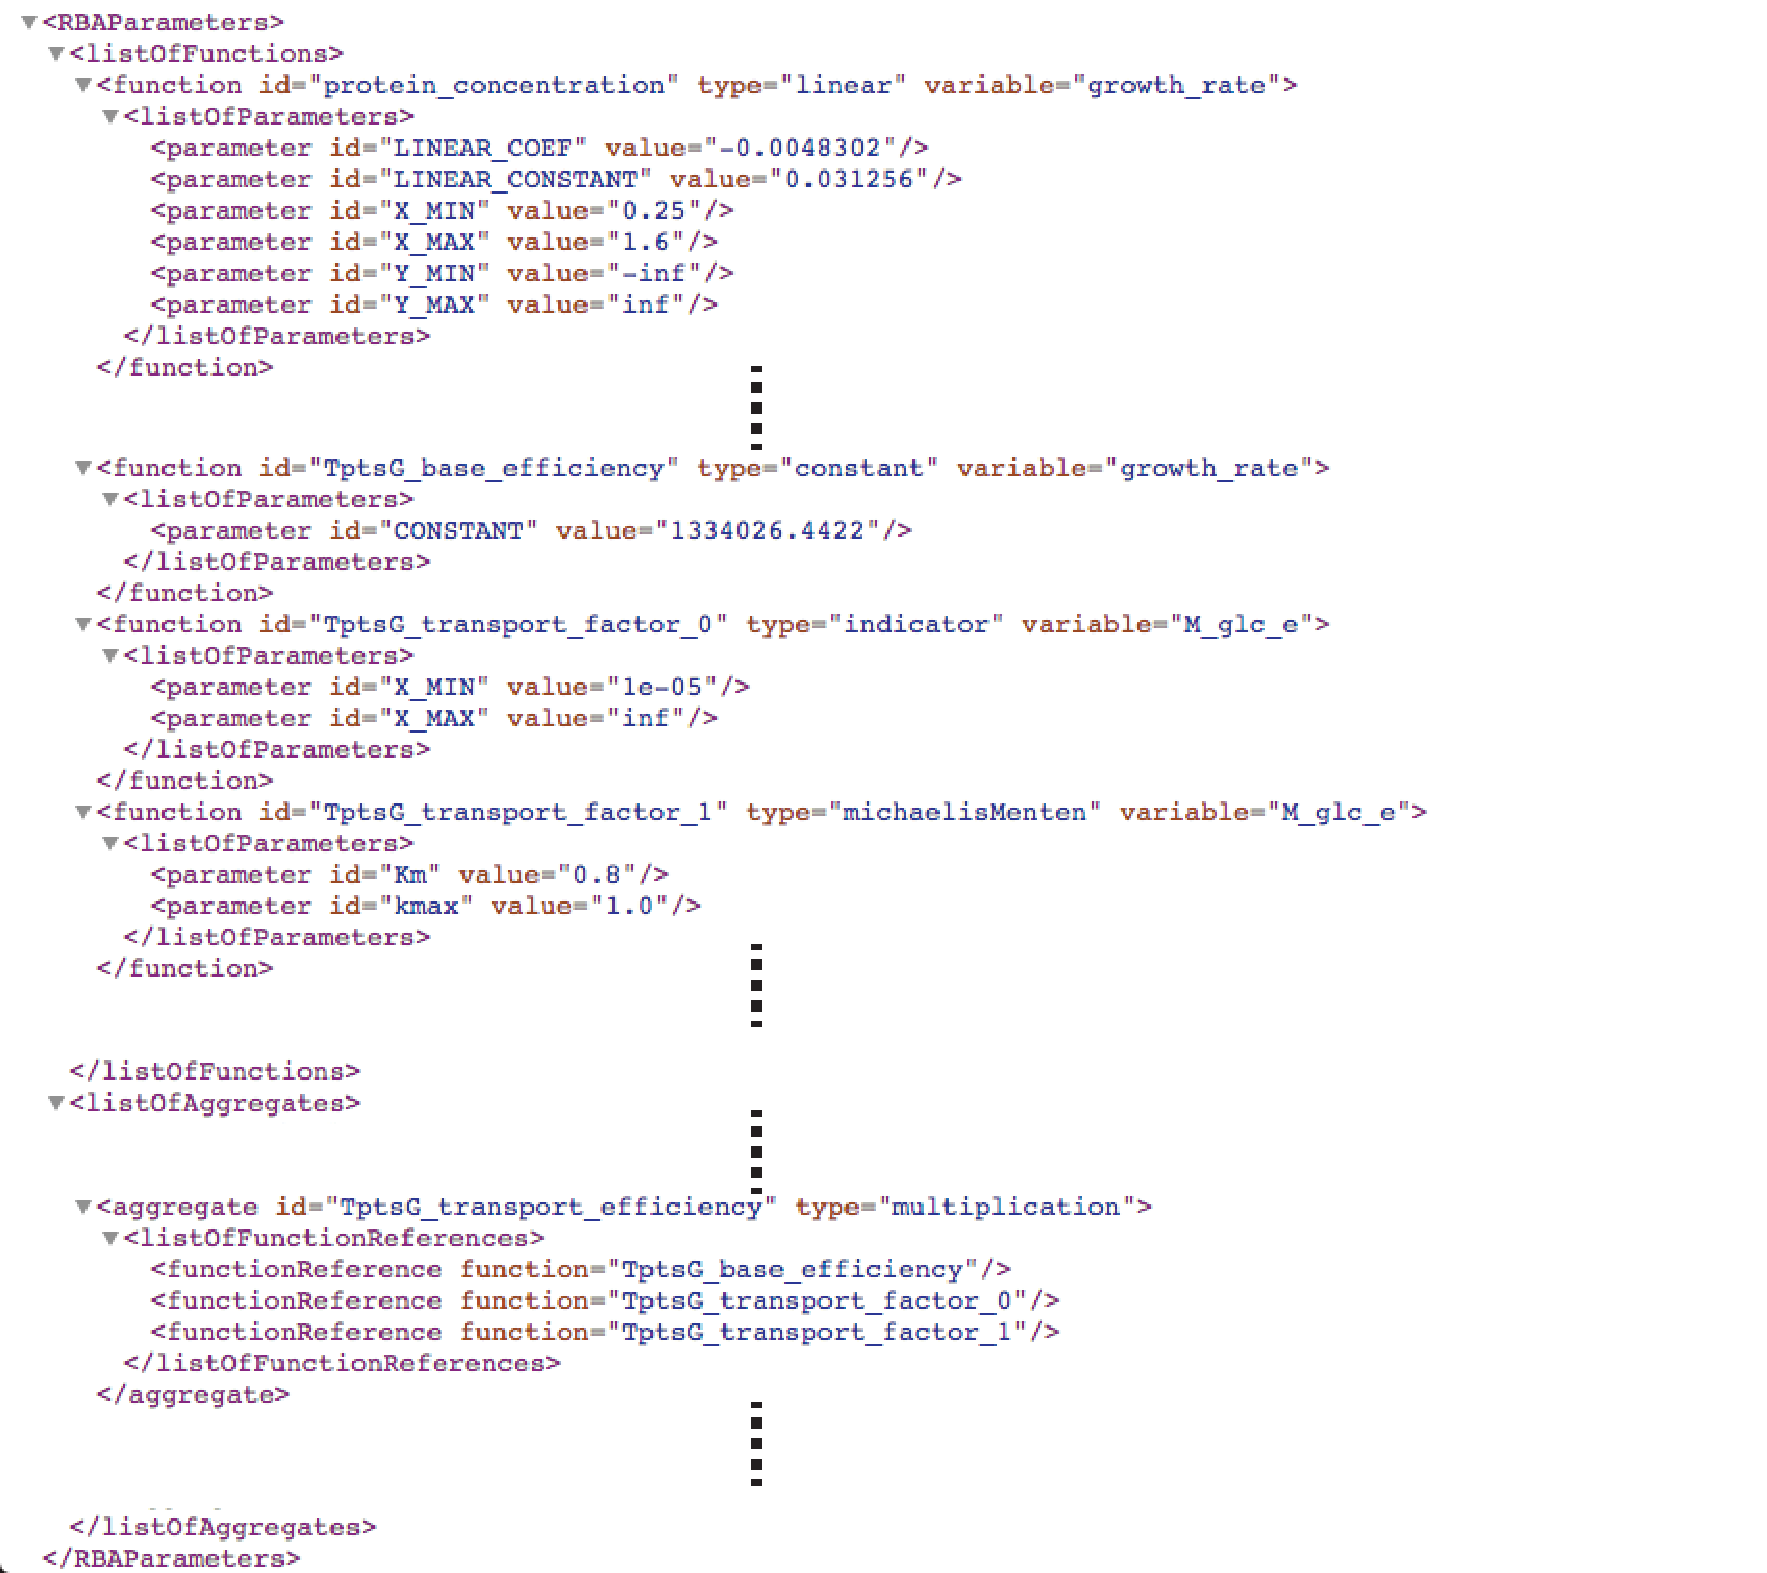
\includegraphics[scale=0.6]{figures/parameters_ex_1}
  \caption{parameters.xml from a hand-curated model for model bacteria \textit{B. subtilis}.
  Large parts of the file were removed for brevity.
  Parameters are defined either as constants, functions (e.g. linear or Michealis-Menten),
  or aggregates, representing the multiplication of functions.
  Functions can be defined in terms of growth rate (the default) or concentration
  of external metabolites.
  Aggregates may contain an arbitrary number of functions,
  and functions in an aggregate can be defined according to different variables
  (growth rate, concentration of different metabolites).}
  \label{fig:parameters_ex_1}
\end{figure}

\begin{figure}
  \centering
  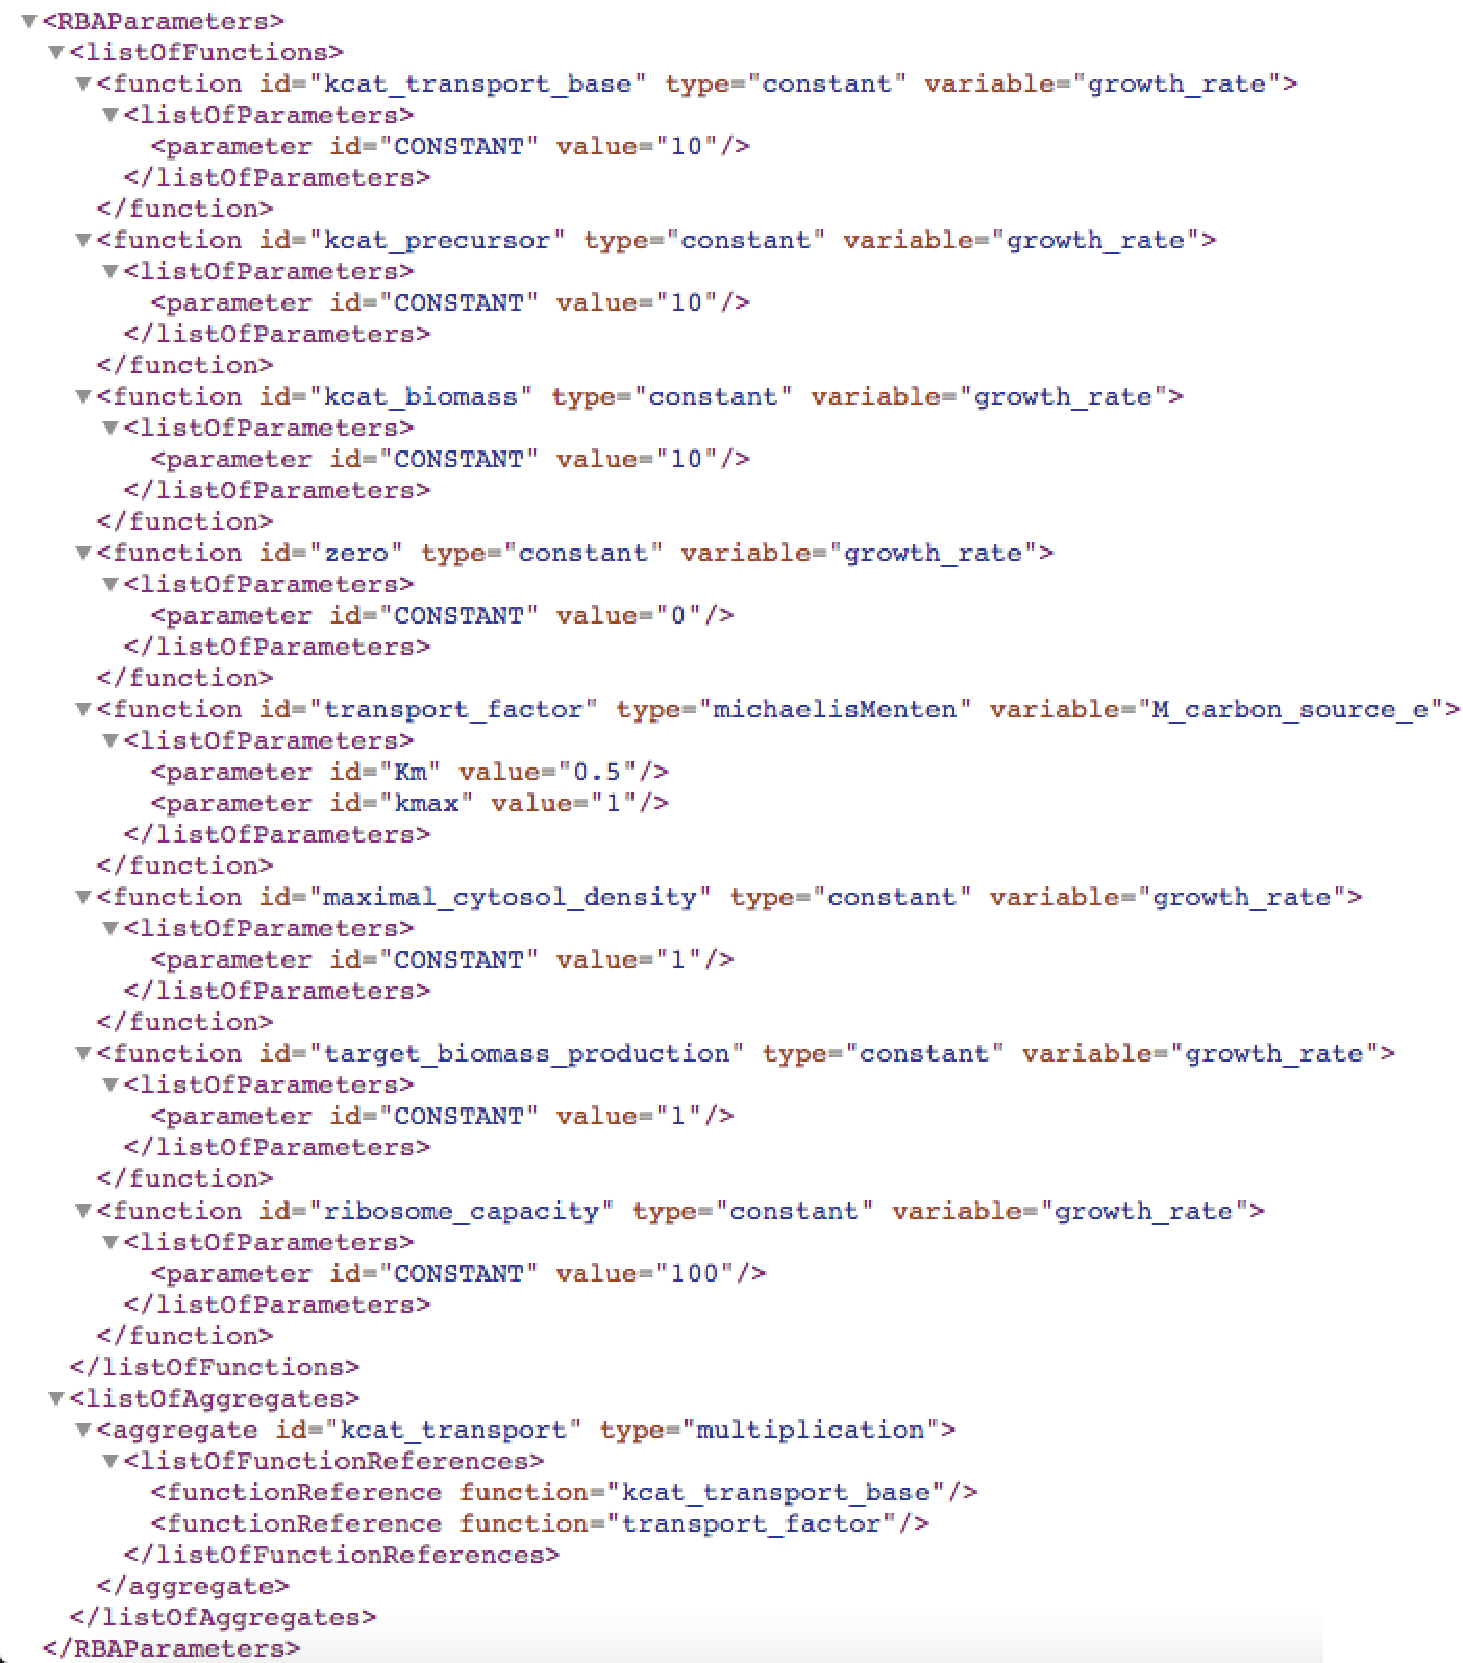
\includegraphics[scale=0.6]{figures/parameters_ex_2}
  \caption{parameters.xml from the minimal model.
  For simplicity, all parameters were defined as constants,
  except for transport terms, which adopt the traditional Michaelis-Menten.}
  \label{fig:parameters_ex_2}
\end{figure}


\section{density.xml}

The density file contains density constraints for the RBA model.

\subsection{Rationale}

A cell can only contain a limited number of macromolecules:
there is a threshold that the total density
(weight per unit volume) cannot exceed.
Every macromolecule has a weight that equals the sum of its components' weights:

\[
  W_i = \sum_{c \in \mathrm{components}} w_c
\]

If we assign every macromolecule a concentration $C_i$, the total density is:

\[
  \sum_{i \in [1..M]} C_i W_i
\]

where $M$ is the total number of macromolecules.

There are two types of density contraints.
In the first case, the density \emph{must} be equal to some density $d$:

\[
  \sum_{i \in [1..M]} C_i W_i = d
\]

Alternatively, the density must not exceed some maximal density $d_{max}$

\[
  \sum_{i \in [1..M]} C_i W_i \leq d_{max}
\]

The XML format allows for equality and inequality constraints by specifying
whether the bound is a lower bound (not applicable for density),
an upper bound (like $d_max$), or a set value (like $d$).

\subsection{RBADensity}
\label{sec:rba_density}

The outermost part of the density file is an instance of class
\rbadensity, shown in Figure~\ref{fig:density_doc}.

\begin{figure}
  \centering
  \includegraphics[scale=0.8]{figures/density_doc}
  \caption{XML structure of density document.}
\label{fig:density_doc}
\end{figure}

\rbadensity{} has no simple attributes.
It includes exactly one instance of \textbf{ListOf} container classes.
All \textbf{ListOf} classes do not have own attributes,
they are merely used to organize a list of instances from another class.

\subsection{TargetDensity}
\label{sec:target_density}

The \targetdensity{} class is used to define density constraints
(Fig.~\ref{fig:density_doc}).
In a RBA model, a density constraint defines how many molecules
a given compartment can contain.
It inherits \targetvalue{} for the constraint definition part.

\paragraph{The \textit{compartment} attribute}
The \textbf{compartment} attribute must match the identifier of a \compartment.


\subsection{TargetValue}
\label{sec:target_value}

The \targetvalue{} class is used to define the sign of an additional RBA
constraint and the value of its second member
(Fig.~\ref{fig:density_doc}).
It is designed to be inherited.
The child class usually holds information about the first member of the
constraint
(\textit{e.g.} compartment for a density constraint,
metabolite for a production constraint).

\paragraph{The \textit{value}, \textit{lowerBound} and \textit{upperBound} attributes}
Every attribute can be left undefined, or
contain the identifier of a \function{} or an \aggregate.

If \textbf{value} is defined, the constraint is an equally constraint.
\textbf{lowerBound} and \textbf{upperBound} are ignored.
If \textbf{value} is undefined, \textbf{lowerBound} (resp. \textbf{upperBound}) defines
a lower bound (resp.\ upper bound) inequality constraint.
Note that \textbf{lowerBound} and \textbf{upperBound} may both be defined, yielding two
separate inequality constraints.

\subsection{Examples}

density.xml is by far the shortest file in an RBA model
(Fig.~\ref{fig:density_ex_1} and \ref{fig:density_ex_2}).
Usually it contains one constraint per compartment,
even though there may be zero or more than one constraint per compartment.
In general, we advise using inequality constraints for greater flexibility
in the model.

\begin{figure}
  \centering
  \includegraphics[scale=0.6]{figures/density_ex_1}
  \caption{density.xml from a hand-curated model for the
  model bacteria \textit{B. subtils}.
  The model defines two density constraints, one per compartment.
  By using upperBound, we define two inquality constraints:
  the density of macromolecules may not exceed parameter
  Cytoplasm\_density in the cytoplasm or Cell\_membrane\_density in the membrane,
  but any lower value is acceptable.}
  \label{fig:density_ex_1}
\end{figure}

\begin{figure}
  \centering
  \includegraphics[scale=0.6]{figures/density_ex_2}
  \caption{density.xml from the minimal model.
  There is only one compartment in the minimal model,
  for which we define an upperBound type density constraint.}
  \label{fig:density_ex_2}
\end{figure}


\section{proteins.xml, rnas.xml and dna.xml}

All these files are base on the same class \rbamacromolecules.


\subsection{RBAMacromolecules}
\label{sec:rba_macromolecules}

The outermost portion of the protein, RNA and DNA files is an instance of class
\rbamacromolecules, shown in Figure~\ref{fig:macromolecules}.

\begin{figure}
  \centering
  \includegraphics[scale=0.8]{figures/macromolecules}
  \caption{XML structure of macromolecule document.}
\label{fig:macromolecules}
\end{figure}

\rbamacromolecules{} has no simple attributes.
It contains exactly one instance of \textbf{ListOfComponents}
and \textbf{ListOfMacromolecules}.


\subsection{Component}
\label{sec:component}

The \component{} class is used to define the components of a \macromolecule{}
(Fig.~\ref{fig:macromolecules}).
For example, these are expected to be amino acids, vitamins and ions for
proteins.
Even if there is a strong connection between metabolic \species and \component{}s,
they are seen as independent entities with separate identifiers \species.
The connection between \species and \component{}s is established in the process file,
where \processingmap{}s define how components are assembled from metabolites.


\paragraph{The \textit{id} attribute}
The \textbf{id} attribute is a string defining the identifier of a component.

\paragraph{The \textit{weight} attribute}
The \textbf{weight} attribute is a real number defining the weight of a
component.
This information is essential for the density constraints.
The weight of a macromolecule is defined as the sum of the weight of its
components.
The weight unit is unspecified, however it should be consistent with the parameters
used in the density constraints.

\paragraph{The \textit{name} and \textit{type} attributes}
The \textbf{name} and \textbf{type} attributes are strings that provide
additional information about the component.
The name is a standard name of the component
(\textit{e.g.} full amino acid name).
The type can be used to distinguish components if necessary
(\textit{e.g.} in amino acids, vitamins, ions).


\subsection{Macromolecule}
\label{sec:macromolecule}

The \macromolecule{} class is used to define macromolecular species
(Fig.~\ref{fig:macromolecules}).
Its composition is given by a \textbf{ListOfComponentReferences}.

\paragraph{The \textit{id} attribute}
The \textbf{id} attribute is a string defining the identifier of
the macromolecule.

\paragraph{The \textit{compartment} attribute}
The \textbf{compartment} attribute must match the identifier of a \compartment.
It represents the compartment where the molecule is thought to be active.


\subsection{ComponentReference}
\label{sec:component_reference}

The \componentreference{} class is used to refer to a \component{}
and associate with it a stoichiometry (Fig.~\ref{fig:macromolecules}).

\paragraph{The \textit{component} attribute}
The \textbf{component} attribute must match the identifier of a \component{}
defined in the same \rbamacromolecules{} instance.

\paragraph{The \textit{stoichiometry} attribute}
The \textbf{stoichiometry} is a positive real number.
It represents the stoichiometry of a \component{}
(typically how often it appears in a \macromolecule,
e.g.\ the number of alanine residues in a protein).


\section{processes.xml}

The process file is used to define constraints related to complex
cellular processes.

\subsection{RBAProcesses}
\label{sec:rba_processes}

The outermost portion of the process file is an instance of class
\rbaprocesses, shown in Figure~\ref{fig:processes_doc}.

\begin{figure}
  \centering
  \includegraphics[scale=0.8]{figures/processes_doc}
  \caption{XML structure of process document.}
\label{fig:processes_doc}
\end{figure}

\rbamacromolecules{} has no simple attributes.
It contains exactly one instance of \textbf{ListOfProcesses}
and \textbf{ListOfComponentMaps}.


\subsection{Process}
\label{sec:process}

The \process{} class is used to define cellular processes
(Fig.~\ref{fig:processes_process}).
Processes cover a wide variety of non-metabolic reactions.

\begin{figure}
  \centering
  \includegraphics[scale=0.8]{figures/processes_process}
  \caption{Class used to store processes.}
\label{fig:processes_process}
\end{figure}

A \process{} revolves around 3 optional substructures.
We encourage you to study existing examples to understand how the different
substructures are used.

The \machinery{} is the molecular entity enabling the process
(\textit{e.g.} ribosome for translation.)
Each machinery unit has a limited production/degradation capacity.
Every target of a process has an intrinsic metabolite cost
(metabolites needed to produce/degrade it and byproducts).
However, if a machinery is defined, there is an additional metabolic cost
to produce the machinery that will enable the production/degradation of the
target.
This is similar to the production of \enzyme{}s in order to catalyze
metabolic \reaction{}s.

\operations{} define the sets of macromolecules that a process
produces or degrades.
A \macromolecule{} can only be produced if it was related to a \process{}.
For example, a protein can only be produced if there is a translation process
where proteins are explicitly listed as a production in \operations{}.
\operations{} break down \macromolecule{}s in metabolic \species{}
and \machinery{} costs.
\operations{} does not define how many molecules of a \macromolecule{}
must be produced.

\targets{} define the fluxes that a process must maintain for the cell
to work properly.
Some fluxes, such as enzyme production, are already enclosed in the base model.
They should not appear in \targets{}.
On the other hand, fluxes such as production of housekeeping proteins need
to be explicitly added to \targets{}.

\paragraph{The \textit{id} attribute}
The \textbf{id} attribute is a string defining the identifier of a process.

\paragraph{The \textit{name} attirbute}
The \textbf{name} attribute is a string that can be used to give the process
a more human understandable name.


\subsection{Machinery}
\label{sec:machinery}

The \machinery{} class defines the machinery used by a process
(Fig.~\ref{fig:processes_process}).
\machinery{} has no simple attributes.
If a \machinery{} is defined, it defines a \emph{capacity constraint}.
Every \machinery{} unit has a metabolic cost defined by a \machinerycomposition.
Every unit also has a capacity defined by a \targetvalue.
The capacity defines how many targets a \machinery{} can process in 1 unit of
time.
Total capacity (base capacity multiplied by number of \machinery{} units)
must always exceed the number of targets produced.


\subsection{MachineryComposition}
\label{sec:machinery_composition}

The \machinerycomposition{} class defines the assembly costs of a complex
molecular machinery (Fig.~\ref{fig:processes_process}).
\machinerycomposition{} has no simple attributes.
It contains two \textbf{ListOfSpeciesReferences}.
One is for reactants, the other for byproducts of the assembly reaction.
Note that in this case, \speciesreference{}s can refer to \emph{both}
metabolic \species{} and \macromolecule{}s.
The assembly reaction should contain obvious components of the machinery,
but also metabolic costs related to assembly (such as ATP/GTP costs)
\emph{unless} these costs are already covered by a process.


\subsection{Operations}
\label{sec:operations}

The \operations{} relates \macromolecule{}s production/degradation to
some given \process{} (Fig.~\ref{fig:processes_process}).
\operations{} has no simple attributes.
It may contain two \textbf{ListOfOperations}, one for production and one for
degradation.


\subsection{Operation}
\label{sec:operation}

The \operations{} class defines how \macromolecule{}s are produced/degraded
(Fig.~\ref{fig:processes_process}).
\operation{} is used to break down \macromolecule{}s into metabolites
by linking them to a \componentmap.

\paragraph{The \textit{componentMap} attribute}
The \textbf{componentMap} attribute must match the identifier of a
\componentmap.
This \componentmap{} will be used to compute the metabolic costs.

\paragraph{The \textit{set} attribute}
The \textbf{set} attribute must refer to a \macromolecule{} set.
Currently, the only acceptable values are \textbf{protein}, \textbf{rna}
and \textbf{dna}.
The set contains the \macromolecule{}s that are being produced/degraded.


\subsection{ComponentMap}
\label{sec:component_map}

The \componentmap{} class is used to convert \macromolecule{}s in
metabolic and machinery costs (Fig.\ref{fig:processes_component_map}).

\begin{figure}
  \centering
  \includegraphics[scale=0.8]{figures/processes_component_map}
  \caption{Class used to store production/degradation of macromolecules.}
\label{fig:processes_component_map}
\end{figure}

There are two types of costs.
The \constantcost{} is a purely metabolic cost.
It contains metabolites that are consumed/produced independent of the
\macromolecule{}'s length (\textit{e.g.} translation initiation).
The \textbf{ListOfCosts} container details \cost{}s depending on the individual
\component{}s of the \macromolecule{}.
They cover metabolic costs used to assemble the \component{} onto the nascent
\macromolecule{}.
They also cover processing costs, \textit{i.e.} how many \machinery{} units
are needed to assemble the \component{}.

\paragraph{The \textit{id} attribute}
The \textbf{id} attribute is a string defining the identifier of a
component map.


\subsection{ConstantCost}
\label{sec:constant_cost}

The \constantcost{} class defines metabolites consumed and byproducts
generated by an assembly process (Fig.\ref{fig:processes_component_map}).
It contains two \textbf{ListOfSpeciesReferences}, one for metabolites
consumed and one for metabolites produced.
Note that in this context, a \speciesreference{} must refer to a
metabolic \species.


\subsection{Cost}
\label{sec:cost}

The \cost{} class defines metabolites consumed and byproducts
generated when assembling a specific \component{}
(Fig.\ref{fig:processes_component_map}).
It contains two \textbf{ListOfSpeciesReferences}, one for metabolites
consumed and one for metabolites produced.
Note that in this context, a \speciesreference{} must refer to a
metabolic \species.
Additionally, it defines a processing cost used in a \machinery{}'s
capacity constraint.

\paragraph{The \textit{component} attribute}
The \textbf{component} attribute is a string that must match the identifier
of a \component{}.

\paragraph{The \textit{processingCost} attribute}
The \textbf{processingCost} attribute is a real value that is used to
compute how many \machinery{} units are needed to assemble the \component{}.
For example, let the processing cost of an amino acid be 1.
The capacity of the \machinery{} (the ribosome) is the number of amino acids
it can assemble per unit of time.
The processing cost allows to compute how many ribosomes are needed
to produce the \component{} and, in the end, the \macromolecule{}
(in this example the number of amino acids divided by the ribosome's capacity).


\subsection{Targets}
\label{sec:targets}

The \targets{} class defines what molecules a \process{} must produce for
the cell to work properly (Fig.~\ref{fig:processes_process}).
\targets{} has no simple attributes.

It contains 3 \textbf{ListOfTargetSpecies}.
These targets allow to define metabolic \species{} or \macromolecule{} fluxes.
One is for production fluxes, another for degradation fluxes.
The last list is for maintaining a target at a given concentration.
The difference with a simple production flux is that keeping a target at a
concentration depends on growth rate.
More precisely, the flux needed to keep the concentration is
the growth rate multiplied by the target concentration.
Note that all fluxes must be positive.
If the target is a \macromolecule, production/degradation can only occur
if an \operations{} section of some \process{} defines how the \macromolecule{}
is actually produced/degraded.

It contains a \textbf{ListOfTargetReactions}.
It is also possible to define target fluxes as reaction fluxes.
These targets add constraints on the flux of a specific metabolic \reaction.
In this case, fluxes may be positive or negative.


\subsection{TargetSpecies}
\label{sec:target_species}

The \targetspecies{} class defines constraints for a species flux
(Fig.~\ref{fig:processes_process}).
It inherits \targetvalue{} for the constraint definition part, allowing for
equality or inequality constraints.

\paragraph{The \textit{species} attribute}
The \textbf{species} attribute is a string that must match the identifier
of a metabolic \species{} or a \macromolecule{}.
Note that the \macromolecule{} must be broken down into metabolite costs
through the \operations{} section of some \process{}.
Otherwise no cost will be applied.


\subsection{TargetReaction}
\label{sec:target_reaction}

The \targetreaction{} class defines constraints for a species flux
(Fig.~\ref{fig:processes_process}).
It inherits \targetvalue{} for the constraint definition part, allowing for
equality or inequality constraints.

\paragraph{The \textit{reaction} attribute}
The \textbf{reaction} attribute is a string that must match the identifier
of a metabolic \reaction{}.


\section{enzymes.xml}

\subsection{Rationale}

The enzyme file is used to define enzyme composition and their catalytic efficiency.
It defines efficiency constraints in the RBA model.
These constraints ensure that a reaction flux is smaller than
the product of efficiency and concentration of the enzyme catalyzing
the reaction.

So far, we have defined two types of basic molecules:
metabolites (in metabolism.xml) and macromolecules (e.g.\ in proteins.xml).
There is a third type of molecule in RBA models called a \emph{molecular machine}.

Molecular machines are composed of metabolites and macromolecules.
Contrary to macromolecules, who share a small pool of components and undergo
complex assembly processes, molecular machines can be composed of any
metabolite or macromolecule, and their assembly is described by a single reaction.
Molecular machines also have a functional role within the cell:
catalyzing metabolic reactions or assisting the assembly of macromolecules.

Enzymes are the simplest molecular machines in RBA models,
their role is to catalyze metabolic reactions (as defined in metabolism.xml).
Process machines are the other molecular machines in RBA models,
their composition is defined identically to enzymes,
but characterizing their role in the assembly of macromolecules,
although similar to the catalysis description, is significantly more complex
(as we will see in processes.xml).

The definition of enzymes contains three parts:
the composition of the enzyme, the reaction the enzyme catalyzes,
and the forward and backward efficiencies of the enzyme.
Only one enzyme can be associated with a reaction:
if a reaction may be catalyzed by several enzyme,
it must be duplicated so that every enzyme can be associated with a separate
reaction.

\subsection{RBAEnzymes}
\label{sec:rba_enzymes}

The outermost part of the metabolism file is an instance of class
\rbaenzymes, shown in Figure~\ref{fig:enzymes_doc}.

\begin{figure}
  \centering
  \includegraphics[scale=0.8]{figures/enzymes_doc}
  \caption{XML structure of enzyme document.}
\label{fig:enzymes_doc}
\end{figure}

\rbaenzymes{} has no simple attributes.
It contains excatly one instance of \textbf{ListOfEnzymes} that is used
to store \enzyme{} information.


\subsection{Enzyme}
\label{sec:enzyme}

The \enzyme{} class is used to define enzymes
(Fig.~\ref{fig:enzymes_doc}).

It contains a \machinerycomposition{} that refers to metabolic \species{}
and \macromolecule{}s composing the \enzyme{}.
Note that the composition can be left unspecified.
In this case, the reaction associated with the enzyme is considered spontaneous.

\paragraph{The \textit{id} attribute}
The \textbf{id} attribute is a string defining the identifier of
the enzyme.

\paragraph{The \textit{reaction} attribute}
The \textbf{reaction} attribute must match the identifier of a metabolic
\reaction.
It represents the reaction catalyzed by the enzyme.
This must be a one-to-one mapping.
A \reaction{} can only have one associated \enzyme{}.
If several \enzyme{}s catalyze the same \reaction{},
the \reaction{} must be duplicated.

\paragraph{The \textit{forwardEfficiency} attribute}
The \textbf{forwardEfficiency} attribute must match the identifier of a
parameter (\function{} or \aggregate{}).
It represents the forward catalytic constant.

\paragraph{The \textit{backwardEfficiency} attribute}
The \textbf{backwardEfficiency} attribute must match the identifier of a
parameter (\function{} or \aggregate{}).
It represents the backward catalytic constant
(only applicable if reaction catalyzed by enzyme is reversible).

\paragraph{The \textit{zeroCost} attribute}
The \textbf{zeroCost} attribute is a boolean value.
If set to true, the reaction associated may occur without having to produce
the enzyme.
If set to false or unspecified, an efficiency constraint is created where the
flux through the reaction has to be smaller than the product of enzyme
efficiency and enzyme concentration.

\subsection{Examples}

A typical enzymes.xml contains a long list of enzymes
(Fig.~\ref{fig:enzymes_ex_1}),
typically one enzyme per metabolic reaction (Fig.~\ref{fig:enzymes_ex_2}).
If a reaction occurs spontaneously, it is not technically necessary to
associate a reaction with it, but RBApy creates an enzyme none-the-less,
showing that the reaction was correctly identified as spontaneous.

The \machinerycomposition{} is identical to a metabolic reaction,
except that it may contain macromolecules, not just metabolites.
In the two examples, enzymes are composed of proteins, with identifiers
defined in proteins.xml.
The reaction could also have included byproducts by defining a \texttt{ListOfProducts}.
A typical example would have been the inclusion of GTP as a reactant and GDP
as a byproduct of the assembly of some enzymes, but we neglected these costs in our models.

Note that the efficiencies are \emph{not} numerical values:
they are parameter identifiers, all parameters of the model being defined in parameters.xml.
Also note that \texttt{zero\_cost} is a flag that is almost always set to false.
Setting it to true effectively removes the enzyme, making the associated reaction
spontaneous.
It was included for retrocompatibility with early RBA versions, where it was
used to counterbalance numerical instabilities.



\begin{figure}
  \centering
  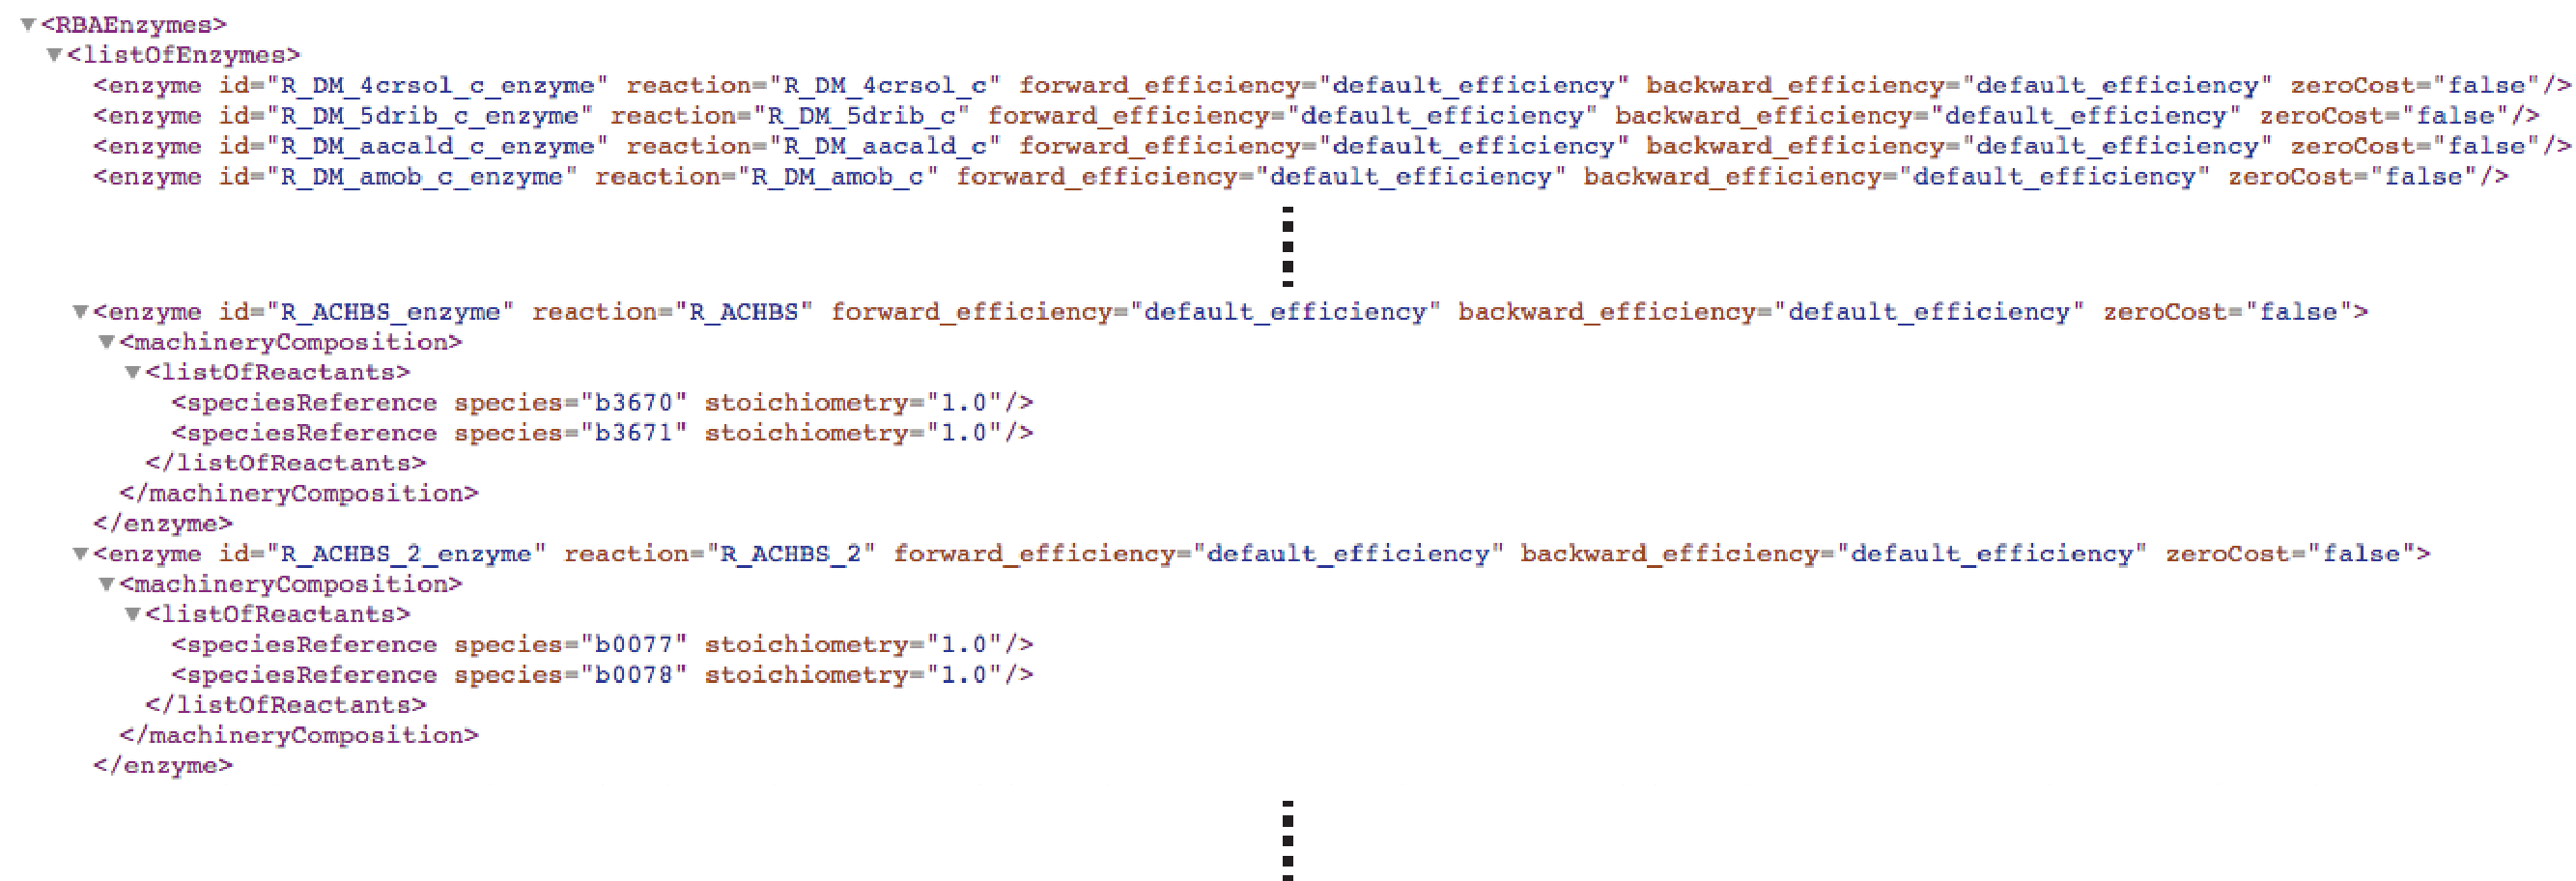
\includegraphics[scale=0.4]{figures/enzymes_ex_1}
  \caption{enzymes.xml from a model automatically generated by RBApy for the
  model bacteria \textit{E. coli}.
  Large chunks of the files were removed for brevity.
  The list starts with 4 enzymes with no composition, indicating that
  the associated reactions occur spontaneously.
  The last two enzymes have different compositions but are associated with
  identical metabolic reactions:
  either of these enzyme may be produced by the cell to catalyze the reaction.}
  \label{fig:enzymes_ex_1}
\end{figure}

\begin{figure}
  \centering
  \includegraphics[scale=0.4]{figures/enzymes_ex_2}
  \caption{enzymes.xml from the minimal model.
  We associate one enzyme with all 3 reactions defined in metabolism.xml.
  Enzymes are defined by using the proteins that we defined in proteins.xml.}
  \label{fig:enzymes_ex_2}
\end{figure}


\section{targets.xml}

The targets file is used to define production and degradation constraints,
i.e. fluxes of metabolic \species{} or \macromolecule{}s that must be maintained
for the cell to be functional.

\subsection{Rationale}

In an RBA model, the production of machines (enzymes and process machines)
is automatically computed to sustain the metabolic fluxes and the production
of macromolecules necessary to achieve optimal growth rate.
However, in order to grow, the cell must produce more than just enzymes and ribosomes.
These production constraints are defined in targets.xml as fluxes or concentrations
that a cell must maintain in order to be functional.

Typical targets include molecules such as DNA, mRNAs, or housekeeping proteins
whose concentration must be maintained at all times.
Structural molecules contained in cell wall for example, must also be
maintained at a constant concentration.
A less obvious example are essential metabolites whose concentration
is high and well regulated, such as NADP/NADPH.\@
Defining a target concentration for NADP forces de novo production of NADP,
otherwise the model assumes that recycling existing NADP is sufficient to achieve any growth rate.
We suggest defining target concentrations for metabolites whenever metabolomic data are available.

In general, targets are defined as concentrations to maintain,
but it's also possible to specify absolute fluxes of production for metabolites or reactions.
A typical reaction flux that must be maintained is the production of maintenance ATP
(ATP used by secondary processes of the cell).

From the XML point of view, the definition of target constraints uses the same structure
as the density constraints.
In particular, the constraints may be equalities
(the concentration must be maintained to that exact value)
or inequalities (the concentration must be maintained between these bounds).

\subsection{RBATargets}
\label{sec:rba_targets}

The outermost part of the process file is an instance of class
\rbatargets, shown in Figure~\ref{fig:targets_doc}.

\begin{figure}
  \centering
  \includegraphics[scale=0.8]{figures/targets_doc}
  \caption{XML structure of target document.}
\label{fig:targets_doc}
\end{figure}

\rbatargets{} has no simple attributes.
It contains 3 \textbf{ListOfTargetSpecies}.
These targets allow to define metabolic \species{} or \macromolecule{} fluxes.
One is for production fluxes, another for degradation fluxes.
The last list is for maintaining a target at a given concentration.
The difference with a simple production flux is that keeping a target at a
concentration depends on growth rate.
More precisely, the flux needed to keep the concentration is
the growth rate multiplied by the target concentration.
Note that all fluxes must be positive.
If the target is a \macromolecule, production/degradation can only occur
if the \processings{} section of some \process{} defines how the
\macromolecule{} is actually produced/degraded.

It contains a \textbf{ListOfTargetReactions}.
It is also possible to define target fluxes as reaction fluxes.
These targets add constraints on the flux of a specific metabolic \reaction.
In this case, fluxes may be positive or negative.


\subsection{TargetSpecies}
\label{sec:target_species}

The \targetspecies{} class defines constraints for a species flux
(Fig.~\ref{fig:targets_doc}).
It inherits \targetvalue{} for the constraint definition part, allowing for
equality or inequality constraints.

\paragraph{The \textit{species} attribute}
The \textbf{species} attribute is a string that must match the identifier
of a metabolic \species{} or a \macromolecule{}.
Note that the \macromolecule{} must be broken down into metabolite costs
through the \processings{} section of some \process{}.
Otherwise no cost will be applied.


\subsection{TargetReaction}
\label{sec:target_reaction}

The \targetreaction{} class defines constraints for a reaction flux
(Fig.~\ref{fig:targets_doc}).
It inherits \targetvalue{} for the constraint definition part, allowing for
equality or inequality constraints.

\paragraph{The \textit{reaction} attribute}
The \textbf{reaction} attribute is a string that must match the identifier
of a metabolic \reaction{}.

\subsection{Examples}

Most targets in an RBA model are concentration targets for DNA production,
mRNA production, housekeeping protein production, de novo metabolite
production, by specifying a concentration that must be maintained
(Fig.~\ref{fig:targets_ex_1} and \ref{fig:targets_ex_2}).

The second class of targets are fluxes related to degradation.
For example, our \textit{B. subtilis} model explicitly accounts for mRNA
degradation.
As a result, there are 3 target fluxes associated with mRNAs:
a flux associated with the target concentration to maintain,
a flux indicating how many molecules are degraded by seconds
(how mRNAs are degraded is defined in processes.xml),
and an absolute production flux that exactly compensates degradation
(Fig.~\ref{fig:targets_ex_1}).

The third class of targets are targets that reference reactions instead of
metabolic species or macromolecules.
Maintenance ATP is one of the most common examples,
but there are a lot of contextual requirements that can be written in this form,
such as flagella movement,
response to stresses such as oxidative stresses causing NADPH consumption.

\begin{figure}
  \centering
  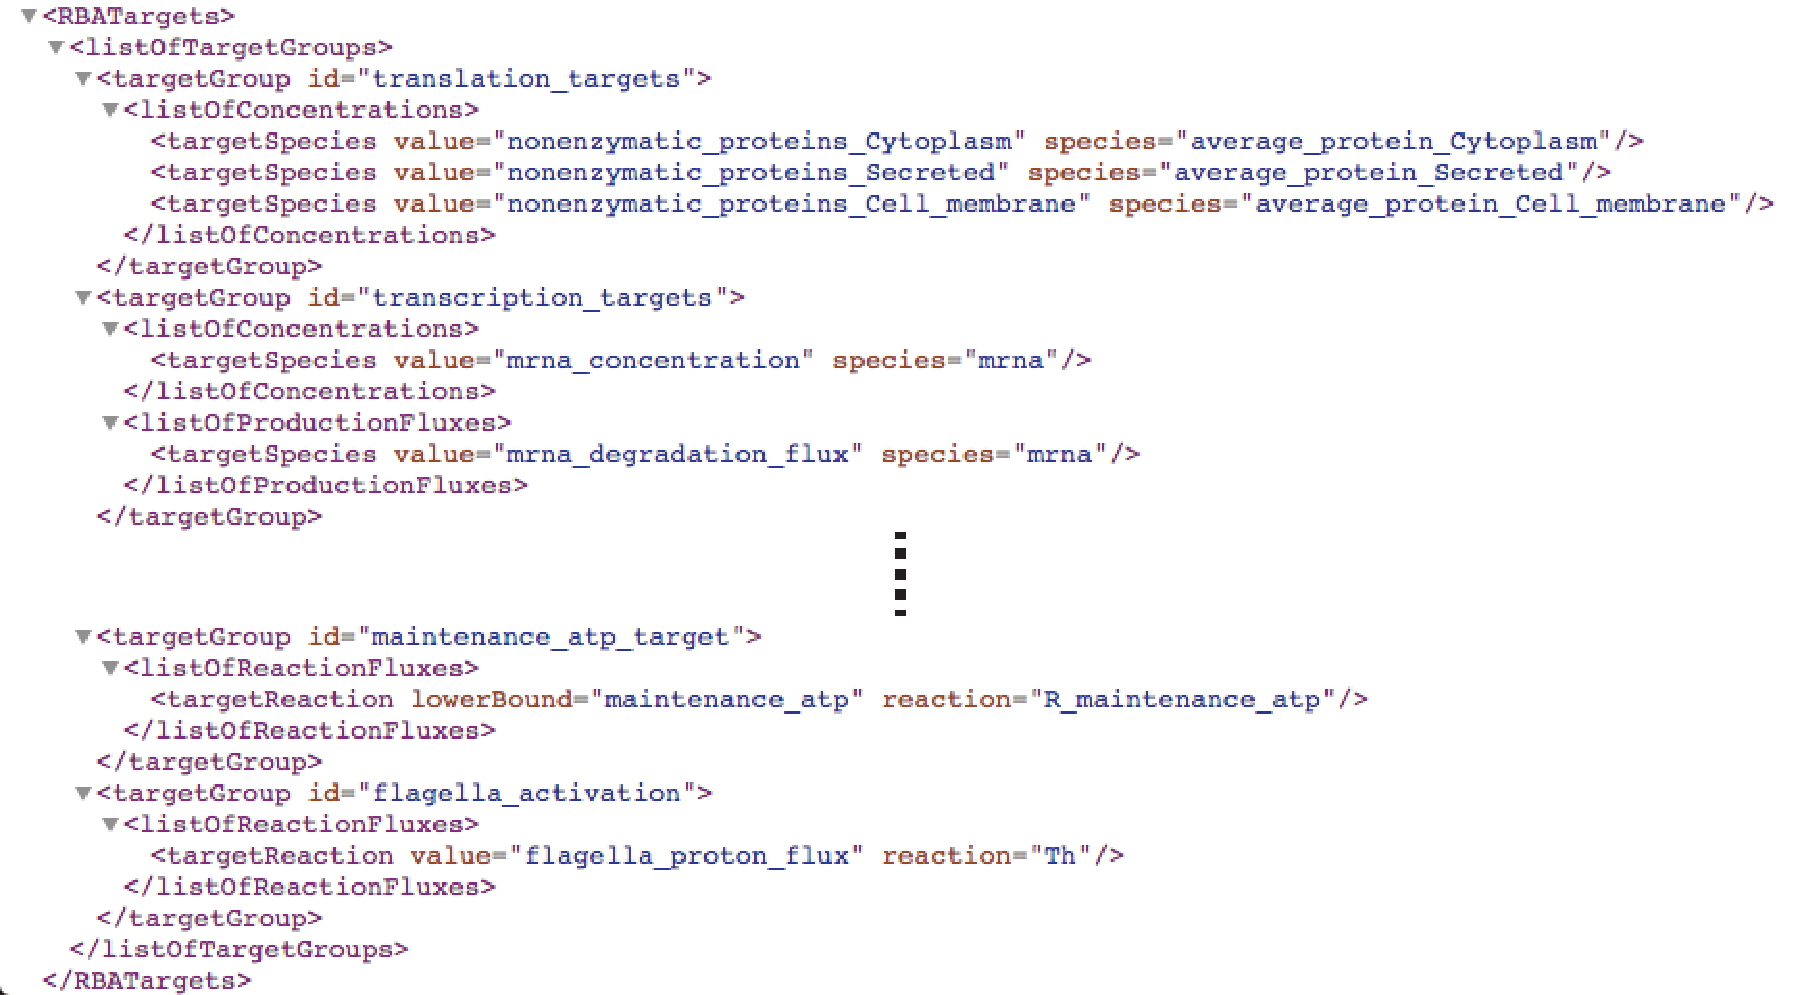
\includegraphics[scale=0.6]{figures/targets_ex_1}
  \caption{targets.xml from a hand-curated model for the
  model bacteria \textit{B. subtilis}.
  Large parts of the files where removed for brevity.
  The first 3 targetSpecies encompass all nonenzymatic proteins that must be
  produced by the cell for housekeeping purposes.
  mRNAs have two production constraints:
  the first contraint defines a flux that must be generated in order to
  maintain their concentration,
  the second constraint defines a flux that must be generated in order to
  compensate degradation (defined later in the file).
  Finally, there are two example of reaction targets:
  a lowerBound for maintainance ATP production,
  and a set bound for the reaction controlling flagella movement.}
  \label{fig:targets_ex_1}
\end{figure}

\begin{figure}
  \centering
  \includegraphics[scale=0.6]{figures/targets_ex_2}
  \caption{targets.xml from the minimal model.
  We pool all non-machine production requirements in a
  generic biomass production requirement.}
  \label{fig:targets_ex_2}
\end{figure}



\end{document}
% ----------------------------------------------------------------
